%%%%%%%%%%%%%%%%%%%%%%%%%%%%%%%%%%%%%%%%%%%%%%%%%%%%%%%%%%%%%%%%%%%%%%%%%%%%%%%%
\documentclass[twocolumn]{revtex4}

%%%%%%%%%%%%%%%%%%%%%%%%%%%%%%%%%%%%%%%%%%%%%%%%%%%%%%%%%%%%%%%%%%%%%%%%%%%%%%%%
% Note that comments begin with a "%" and are not turned into text in the .pdf
% document.
%%%%%%%%%%%%%%%%%%%%%%%%%%%%%%%%%%%%%%%%%%%%%%%%%%%%%%%%%%%%%%%%%%%%%%%%%%%%%%%%

%%%%%%%%%%%%%%%%%%%%%%%%%%%%%%%%%%%%%%%%%%%%%%%%%%%%%%%%%%%%%%%%%%%%%%%%%%%%%%%%
% Include some extra packages.
%%%%%%%%%%%%%%%%%%%%%%%%%%%%%%%%%%%%%%%%%%%%%%%%%%%%%%%%%%%%%%%%%%%%%%%%%%%%%%%%
\usepackage[]{graphicx}

%%%%%%%%%%%%%%%%%%%%%%%%%%%%%%%%%%%%%%%%%%%%%%%%%%%%%%%%%%%%%%%%%%%%%%%%%%%%%%%%

%%%%%%%%%%%%%%%%%%%%%%%%%%%%%%%%%%%%%%%%%%%%%%%%%%%%%%%%%%%%%%%%%%%%%%%%%%%%%%%%
\begin{document}
%%%%%%%%%%%%%%%%%%%%%%%%%%%%%%%%%%%%%%%%%%%%%%%%%%%%%%%%%%%%%%%%%%%%%%%%%%%%%%%%
\title{
Journal article
}

\author{M.~Bellis}
\author{R.~Feynman}
\affiliation{Siena College, Loudonville, NY}

\date{\today}

\begin{abstract}


We had to make a graph of a velociraptor moving 18 m/s and a person moving in the same direction at 3 m/s with a 30 meter head start. From the graph we had to find where the person and the velociraptor would meet, and where the velociraptor and man would be when the velociraptor was almost exactly 1 meter behind it. Finally we had to see if the velociraptor would be able to kill the man using conditionals and percentages given to us. The velociraptor had three chances, the first there was a 20% possibility of the man being caught, then a 15% chance, then a 7% chance. If the man was still alive after the three tries he would have gotten away successfully. 
\end{abstract}

\maketitle
%%%%%%%%%%%%%%%%%%%%%%%%%%%%%%%%%%%%%%%%%%%%%%%%%%%%%%%%%%%%%%%%%%%%%%%%%%%%%%%%

%%%%%%%%%%%%%%%%%%%%%%%%%%%%%%%%%%%%%%%%%%%%%%%%%%%%%%%%%%%%%%%%%%%%%%%%%%%%%%%%
\section{Introduction}
%%%%%%%%%%%%%%%%%%%%%%%%%%%%%%%%%%%%%%%%%%%%%%%%%%%%%%%%%%%%%%%%%%%%%%%%%%%%%%%%
For the first question I just coded a graph that had x, y1, and y2. y1 was 18*x and y2 was 30 + 3*x. For the second question I used the range function to find the ranges of y1 and y2, and expanded it to show when y1 was equal to y2. For the third question I once again used the range function but now included y2[i] - 1 < y1[i], this would show me when the difference in y1 and y2 was less than 1 when y1 was smaller, and when y1 was just larger over all. For the fourth question i used conditionals to see how often the man would die and then I ran the cell 100 times.

%%%%%%%%%%%%%%%%%%%%%%%%%%%%%%%%%%%%%%%%%%%%%%%%%%%%%%%%%%%%%%%%%%%%%%%%%%%%%%%%
\section{Other stuff}

$$v = x_0 + v_0 t$$
$$\delta x = (v_0 t + v) / 2 + t$$
This is the equation I used when solving for position.
%%%%%%%%%%%%%%%%%%%%%%%%%%%%%%%%%%%%%%%%%%%%%%%%%%%%%%%%%%%%%%%%%%%%%%%%%%%%%%%%
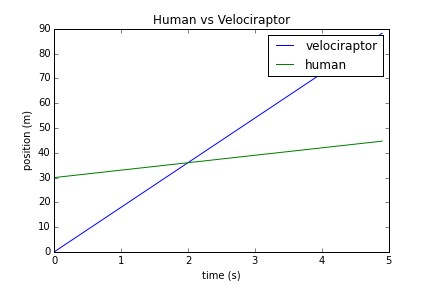
\includegraphics[width=0.5\textwidth]{foo.png}
%%%%%%%%%%%%%%%%%%%%%%%%%%%%%%%%%%%%%%%%%%%%%%%%%%%%%%%%%%%%%%%%%%%%%%%%%%%%%%%%
\end{document}
%%%%%%%%%%%%%%%%%%%%%%%%%%%%%%%%%%%%%%%%%%%%%%%%%%%%%%%%%%%%%%%%%%%%%%%%%%%%%%%%
